\documentclass[a4paper,12pt]{article} % Choose paper size and font size
\usepackage[utf8]{inputenc}  % Support for UTF-8 characters
\usepackage{amsmath}         % Mathematical features
\usepackage{graphicx}   

\title{This is a book}
\author{
  Mabel Liu\thanks{she is responsible for writing} \and
  Leslie Liu\thanks{she is responsible for big data}
}

\date{\today}

\begin{document}
\maketitle

\begin{abstract}
This is a good book.
\end{abstract}

\section{Introduction}
This is book introduces a good story about book loving.
\subsection{Background}
This is about the book of book loving.
\section{Methodology}
This articel will use mathematics and statistics to take the numbers of book loving.
\( a^2 + b^2 = c^2 \).
\section{Results}
This book is a good book how to prove it.

\begin{figure}[h]
  \centering
  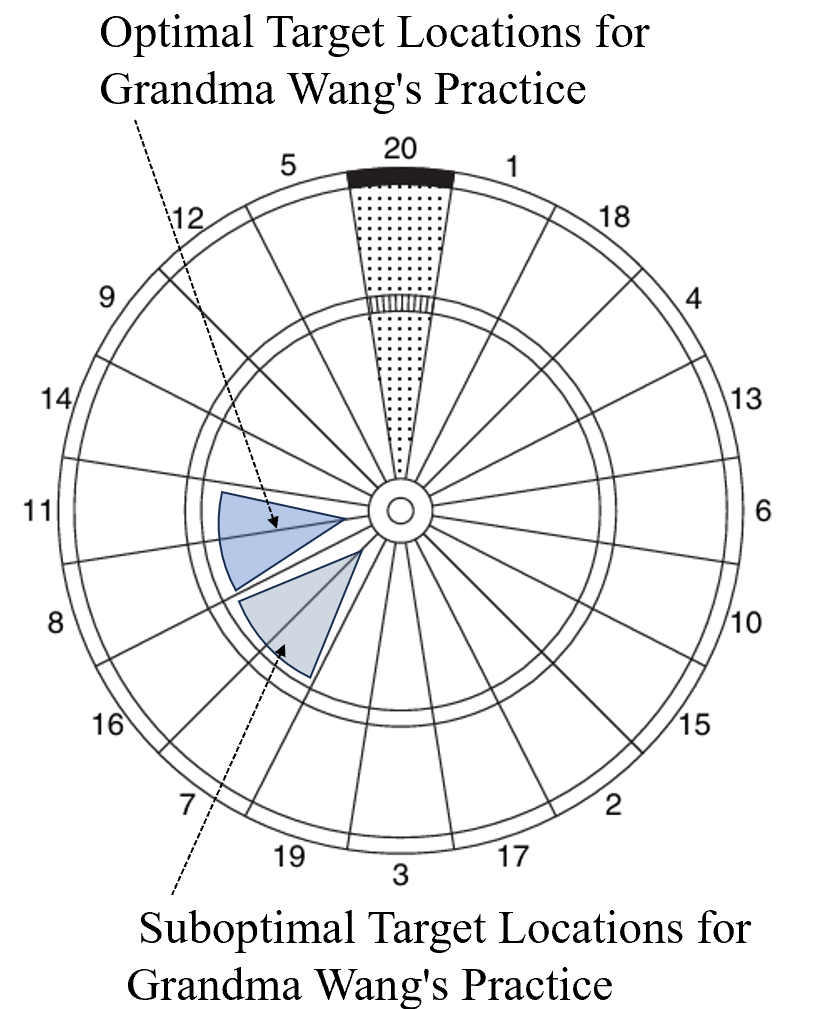
\includegraphics[width=0.5\textwidth]{example.jpg}
  \caption{example.}
  \label{fig:sample}
\end{figure}

\begin{table}[h]
\centering
\begin{tabular}{|c|c|c|}
\hline
Col 1 & Col 2 & Col 3 \\
\hline
A & B & C \\
\hline
1&2&3\\
\hline
\end{tabular}
\caption{A simple table.}
\end{table}
\section{Conclusion}
Everyone love the book of book loving.

\begin{thebibliography}{9}
\bibitem{ref1} Mabel Liu, \textit{This is a book 1 }, International press, 2025.

\bibitem{ref2} Mabel Liu, \textit{This is a book 2 }, AMSA Journal, Vol. 9 (No. 2), 2024

\end{thebibliography}

\end{document}




 